\documentclass{standalone}
\usepackage{tikz}
\usetikzlibrary{patterns, positioning}


\begin{document}
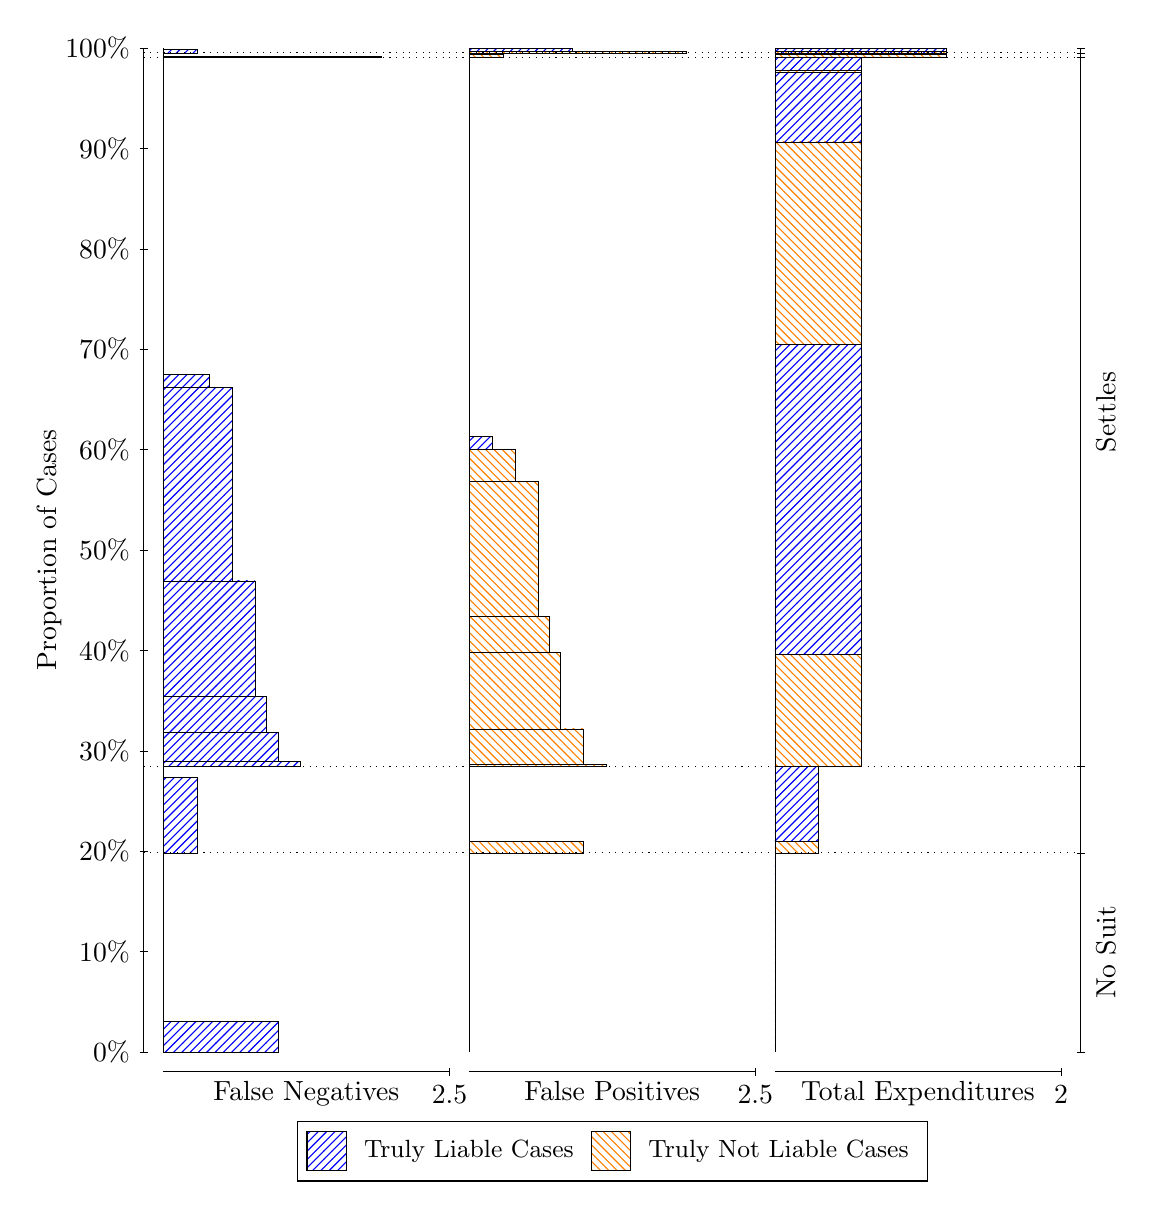
\begin{tikzpicture}
\draw[black, very thin] (1.5,1.75) -- (1.5,14.5);
\node[rotate=90, text=black, anchor=center] at (0.3, 8.125) {Proportion of Cases};
\draw[black, very thin] (1.45,1.75) -- (1.55,1.75);
\node[text=black, anchor=east] at (1.45, 1.75) {0\%};
\draw[black, very thin] (1.45,3.025) -- (1.55,3.025);
\node[text=black, anchor=east] at (1.45, 3.025) {10\%};
\draw[black, very thin] (1.45,4.3) -- (1.55,4.3);
\node[text=black, anchor=east] at (1.45, 4.3) {20\%};
\draw[black, very thin] (1.45,5.575) -- (1.55,5.575);
\node[text=black, anchor=east] at (1.45, 5.575) {30\%};
\draw[black, very thin] (1.45,6.85) -- (1.55,6.85);
\node[text=black, anchor=east] at (1.45, 6.85) {40\%};
\draw[black, very thin] (1.45,8.125) -- (1.55,8.125);
\node[text=black, anchor=east] at (1.45, 8.125) {50\%};
\draw[black, very thin] (1.45,9.4) -- (1.55,9.4);
\node[text=black, anchor=east] at (1.45, 9.4) {60\%};
\draw[black, very thin] (1.45,10.675) -- (1.55,10.675);
\node[text=black, anchor=east] at (1.45, 10.675) {70\%};
\draw[black, very thin] (1.45,11.95) -- (1.55,11.95);
\node[text=black, anchor=east] at (1.45, 11.95) {80\%};
\draw[black, very thin] (1.45,13.225) -- (1.55,13.225);
\node[text=black, anchor=east] at (1.45, 13.225) {90\%};
\draw[black, very thin] (1.45,14.5) -- (1.55,14.5);
\node[text=black, anchor=east] at (1.45, 14.5) {100\%};

\draw[black, very thin] (13.4,1.75) -- (13.4,14.5);
\draw[black, very thin] (13.35,1.75) -- (13.45,1.75);
\node[anchor=west] at (13.35, 1.75) {};
\draw[black, very thin] (13.35,4.2786) -- (13.45,4.2786);
\node[anchor=west] at (13.35, 4.2786) {};
\draw[black, very thin] (13.35,5.3794) -- (13.45,5.3794);
\node[anchor=west] at (13.35, 5.3794) {};
\draw[black, very thin] (13.35,14.377) -- (13.45,14.377);
\node[anchor=west] at (13.35, 14.377) {};
\draw[black, very thin] (13.35,14.439) -- (13.45,14.439);
\node[anchor=west] at (13.35, 14.439) {};
\draw[black, very thin] (13.35,14.5) -- (13.45,14.5);
\node[anchor=west] at (13.35, 14.5) {};

\draw[black, very thin, pattern color=blue, pattern=north east lines] (1.75,1.75) rectangle (3.2033,2.1349);
\draw[black, very thin, pattern color=orange, pattern=north west lines] (1.75,2.1349) rectangle (1.75,4.2786);
\draw[black, very thin, pattern color=blue, pattern=north east lines] (1.75,4.2786) rectangle (2.186,5.2348);
\draw[black, very thin, pattern color=orange, pattern=north west lines] (1.75,5.2348) rectangle (1.75,5.3794);
\draw[black, very thin, pattern color=blue, pattern=north east lines] (1.75,5.3794) rectangle (3.494,5.4415);
\draw[black, very thin, pattern color=blue, pattern=north east lines] (1.75,5.4415) rectangle (3.2033,5.8098);
\draw[black, very thin, pattern color=blue, pattern=north east lines] (1.75,5.8098) rectangle (3.058,6.2644);
\draw[black, very thin, pattern color=blue, pattern=north east lines] (1.75,6.2644) rectangle (2.9127,7.7333);
\draw[black, very thin, pattern color=blue, pattern=north east lines] (1.75,7.7333) rectangle (2.622,10.192);
\draw[black, very thin, pattern color=blue, pattern=north east lines] (1.75,10.192) rectangle (2.3313,10.353);
\draw[black, very thin, pattern color=orange, pattern=north west lines] (1.75,10.353) rectangle (1.75,14.377);
\draw[black, very thin, pattern color=blue, pattern=north east lines] (1.75,14.377) rectangle (4.5113,14.397);
\draw[black, very thin, pattern color=orange, pattern=north west lines] (1.75,14.397) rectangle (1.75,14.439);
\draw[black, very thin, pattern color=blue, pattern=north east lines] (1.75,14.439) rectangle (2.186,14.48);
\draw[black, very thin, pattern color=orange, pattern=north west lines] (1.75,14.48) rectangle (1.75,14.5);
\draw[black, very thin, pattern color=orange, pattern=north west lines] (5.6333,1.75) rectangle (5.6333,3.8937);
\draw[black, very thin, pattern color=blue, pattern=north east lines] (5.6333,3.8937) rectangle (5.6333,4.2786);
\draw[black, very thin, pattern color=orange, pattern=north west lines] (5.6333,4.2786) rectangle (7.0867,4.4231);
\draw[black, very thin, pattern color=blue, pattern=north east lines] (5.6333,4.4231) rectangle (5.6333,5.3794);
\draw[black, very thin, pattern color=orange, pattern=north west lines] (5.6333,5.3794) rectangle (7.3773,5.4029);
\draw[black, very thin, pattern color=orange, pattern=north west lines] (5.6333,5.4029) rectangle (7.0867,5.8519);
\draw[black, very thin, pattern color=orange, pattern=north west lines] (5.6333,5.8519) rectangle (6.796,6.8275);
\draw[black, very thin, pattern color=orange, pattern=north west lines] (5.6333,6.8275) rectangle (6.6507,7.2792);
\draw[black, very thin, pattern color=orange, pattern=north west lines] (5.6333,7.2792) rectangle (6.5053,8.997);
\draw[black, very thin, pattern color=orange, pattern=north west lines] (5.6333,8.997) rectangle (6.2147,9.4034);
\draw[black, very thin, pattern color=blue, pattern=north east lines] (5.6333,9.4034) rectangle (5.924,9.5637);
\draw[black, very thin, pattern color=blue, pattern=north east lines] (5.6333,9.5637) rectangle (5.6333,14.377);
\draw[black, very thin, pattern color=orange, pattern=north west lines] (5.6333,14.377) rectangle (6.0693,14.419);
\draw[black, very thin, pattern color=blue, pattern=north east lines] (5.6333,14.419) rectangle (5.6333,14.439);
\draw[black, very thin, pattern color=orange, pattern=north west lines] (5.6333,14.439) rectangle (8.3947,14.46);
\draw[black, very thin, pattern color=blue, pattern=north east lines] (5.6333,14.46) rectangle (6.9413,14.5);
\draw[black, very thin, pattern color=orange, pattern=north west lines] (9.5167,1.75) rectangle (9.5167,3.8937);
\draw[black, very thin, pattern color=blue, pattern=north east lines] (9.5167,3.8937) rectangle (9.5167,4.2786);
\draw[black, very thin, pattern color=orange, pattern=north west lines] (9.5167,4.2786) rectangle (10.062,4.4231);
\draw[black, very thin, pattern color=blue, pattern=north east lines] (9.5167,4.4231) rectangle (10.062,5.3794);
\draw[black, very thin, pattern color=orange, pattern=north west lines] (9.5167,5.3794) rectangle (10.607,6.8039);
\draw[black, very thin, pattern color=blue, pattern=north east lines] (9.5167,6.8039) rectangle (10.607,10.732);
\draw[black, very thin, pattern color=orange, pattern=north west lines] (9.5167,10.732) rectangle (10.607,13.308);
\draw[black, very thin, pattern color=blue, pattern=north east lines] (9.5167,13.308) rectangle (10.607,14.193);
\draw[black, very thin, pattern color=orange, pattern=north west lines] (9.5167,14.193) rectangle (10.607,14.216);
\draw[black, very thin, pattern color=blue, pattern=north east lines] (9.5167,14.216) rectangle (10.607,14.377);
\draw[black, very thin, pattern color=orange, pattern=north west lines] (9.5167,14.377) rectangle (11.697,14.419);
\draw[black, very thin, pattern color=blue, pattern=north east lines] (9.5167,14.419) rectangle (11.697,14.439);
\draw[black, very thin, pattern color=orange, pattern=north west lines] (9.5167,14.439) rectangle (11.697,14.46);
\draw[black, very thin, pattern color=blue, pattern=north east lines] (9.5167,14.46) rectangle (11.697,14.5);
\draw[black, dotted] (1.5,4.2786) -- (13.4,4.2786);
\draw[black, dotted] (1.5,5.3794) -- (13.4,5.3794);
\draw[black, dotted] (1.5,14.377) -- (13.4,14.377);
\draw[black, dotted] (1.5,14.439) -- (13.4,14.439);
\draw[black, very thin] (1.75,1.5) -- (5.3833,1.5);
\node[text=black, anchor=north] at (3.5667, 1.5) {False Negatives};
\draw[black, very thin] (5.3833,1.45) -- (5.3833,1.55);
\node[text=black, anchor=north] at (5.3833, 1.45) {2.5};

\draw[black, very thin] (5.6333,1.5) -- (9.2667,1.5);
\node[text=black, anchor=north] at (7.45, 1.5) {False Positives};
\draw[black, very thin] (9.2667,1.45) -- (9.2667,1.55);
\node[text=black, anchor=north] at (9.2667, 1.45) {2.5};

\draw[black, very thin] (9.5167,1.5) -- (13.15,1.5);
\node[text=black, anchor=north] at (11.333, 1.5) {Total Expenditures};
\draw[black, very thin] (13.15,1.45) -- (13.15,1.55);
\node[text=black, anchor=north] at (13.15, 1.45) {2};

\node[text=black, centered, rotate=90] at (13.72, 3.0143) {No Suit};

\node[text=black, centered, rotate=90] at (13.72, 9.878) {Settles};



\draw (7.449999999999999,1.5) node[draw=none] (baseCoordinate) {};
\begin{scope}[align=center]
        \matrix[scale=0.5, draw=black, below=0.5cm of baseCoordinate, nodes={draw}, column sep=0.1cm]{
            \node[rectangle, draw, minimum width=0.5cm, minimum height=0.5cm, pattern color=blue, pattern=north east lines] {}; &
            \node[draw=none, font=\small, text=black] (B) {Truly Liable Cases}; &
            \node[rectangle, draw, minimum width=0.5cm, minimum height=0.5cm, pattern color=orange, pattern=north west lines] {}; &
            \node[draw=none, font=\small, text=black] (B) {Truly Not Liable Cases}; \\
            };
\end{scope}

\end{tikzpicture}
\end{document}